% Traceability: manual-local recurrent field chapter.
\subsection{Recurrent systems}

\subsubsection{Recurrent ring witness}
\label{man:recurrent-ring-witness}
\colabbadge{manual/notebooks/04e_recurrent_ring.ipynb}

\begin{table}[H]
\centering
\caption{Recurrent retained-extraction declaration.}
\label{tab:recurrent-retention}
\begin{threeparttable}
\begin{tabularx}{\linewidth}{@{}lX@{}}
\toprule
Item & Declaration \\
\midrule
Parent field & cited recurrent AO field \\
Retained extraction & three-node recurrent ring \\
Omitted context & non-ring recurrent context \\
First refinement & extended recurrent network \\
Validity window & cited recurrent row \\
Residual witness & pending until refinement row is computed \\
\bottomrule
\end{tabularx}
\end{threeparttable}
\end{table}

A cited recurrent-ring row is fixed first and then displayed as a compact recurrent-system witness.

\begin{table}[H]
\centering
\caption{Recurrent ring witness row.}
\label{tab:recurrent-ring-witness-row}
\begin{threeparttable}
\small
\pgfplotstabletypeset[
  columns={row_id,topology,Rloss_trit_per_bip,B_star_mode_bip,Lambda_hat_ticks,Rloss_biz_derived},
  columns/row_id/.style={column name=Row,string type,column type=l},
  columns/topology/.style={column name=Topology,string type,column type=l},
  columns/Rloss_trit_per_bip/.style={column name={$R_{\mathrm{loss}}$ [\(\mathrm{trit}/\mathrm{bip}_0\)]},fixed,precision=6},
  columns/B_star_mode_bip/.style={column name={$B^*$ [\(\mathrm{bip}_0\)]},fixed,precision=0},
  columns/Lambda_hat_ticks/.style={column name={$\widehat\Lambda$ [ticks]},fixed,precision=0},
  columns/Rloss_biz_derived/.style={column name={$R^{(\mathrm{biz}_0)}_{\mathrm{loss}}$ [\(\mathrm{biz}_0\)]},fixed,precision=6}
]{data/temporal/01_recurrent_ring_summary.csv}
\ManualTableNote{This compact display reuses the cited recurrent-ring row as a recurrent-system witness across scales.}
\end{threeparttable}
\end{table}

\begin{figure}[H]
\centering
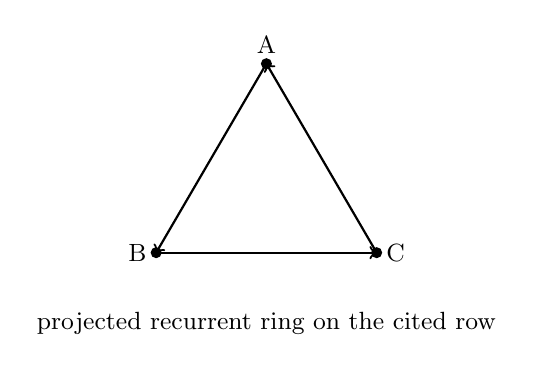
\begin{tikzpicture}[x=1cm,y=1cm, every node/.style={font=\small}]
  \coordinate (A) at (0,1.6);
  \coordinate (B) at (-1.4,-0.8);
  \coordinate (C) at (1.4,-0.8);
  \draw[thick,->] (A) -- (B);
  \draw[thick,->] (B) -- (C);
  \draw[thick,->] (C) -- (A);
  \fill (A) circle (2pt) node[above] {A};
  \fill (B) circle (2pt) node[left] {B};
  \fill (C) circle (2pt) node[right] {C};
  \node at (0,-1.7) {projected recurrent ring on the cited row};
\end{tikzpicture}
\caption{Recurrent ring witness.}
\label{fig:recurrent-ring-witness}
\end{figure}

The cited recurrent row carries the CK-mismatch and cut-residual diagnostics used to distinguish recurrent projection effects from kernel bias.


\subsubsection{Driven chirality-flip toy model}
\label{man:driven-chirality-flip-toy}
\colabbadge{manual/notebooks/04e_driven_chirality_flip_toy.ipynb}

\begin{table}[H]
\centering
\caption{Driven chirality toy retained-extraction declaration.}
\label{tab:chirality-toy-retention}
\begin{threeparttable}
\begin{tabularx}{\linewidth}{@{}lX@{}}
\toprule
Item & Declaration \\
\midrule
Parent field & toy recurrent collision field \\
Retained extraction & driven duon reclosure schedule \\
Omitted context & non-toy recurrent context and benchmark fields \\
First refinement & backlog/reconciliation-driven recurrent field \\
Validity window & simulation window only \\
Residual witness & qualitative; support-only until exact refinement exists \\
\bottomrule
\end{tabularx}
\ManualTableNote{This toy is support-only; it is not theorem evidence and not a cross-scale benchmark witness.}
\end{threeparttable}
\end{table}

This is a support-only toy model. It is not theorem evidence and not a cross-scale benchmark witness. The companion notebook tracks chirality flips, push/pull response, and mean chirality polarization under unbiased and driven reclosure schedules.

\begin{table}[H]
\centering
\caption{Driven chirality-flip toy model summary.}
\label{tab:driven-chirality-flip-toy}
\begin{threeparttable}
\small
\begin{tabularx}{\linewidth}{@{}lrrrrr@{}}
\toprule
Scenario & Collisions & Flips & Flips / collision & Peak $|\chi|$ & Mean push/pull \\
\midrule
No external bias & 106051 & 808 & 0.00762 & 0.24 & 0.0550 \\
Driven bias & 130014 & 1173 & 0.00902 & 0.36 & -0.0001 \\
\bottomrule
\end{tabularx}
\ManualTableNote{The driven run increases both total collisions and flip probability per collision relative to the unbiased run. The companion notebook also displays the push/pull and flip-event diagnostics.}
\end{threeparttable}
\end{table}

\begin{figure}[H]
\centering
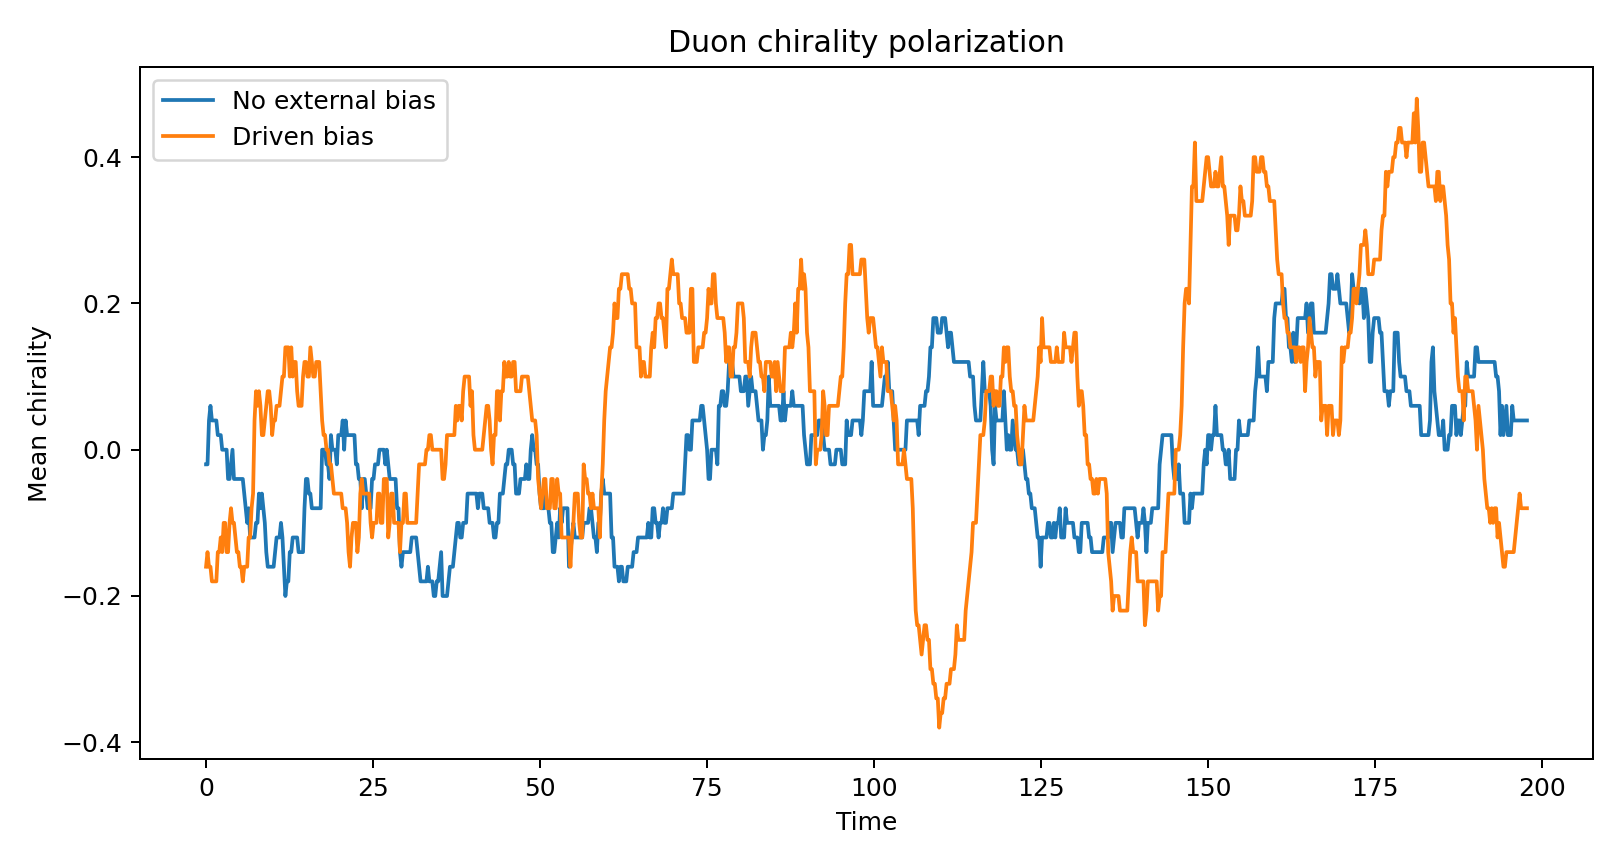
\includegraphics[width=0.82\linewidth]{figures/recurrent/01_duon_chirality_polarization.png}
\caption{Driven chirality polarization in the recurrent collision toy model.}
\label{fig:driven-chirality-polarization}
\end{figure}

The driven schedule produces larger chirality excursions and a higher flip rate per collision than the unbiased run.
